
% Single column for now
%\documentclass[conference]{IEEEtran}
\documentclass{article}

\usepackage{graphicx}
\graphicspath{{figures/}}
\DeclareGraphicsExtensions{.pdf,.jpeg,.png,.eps}
\usepackage[cmex10]{amsmath}
\usepackage{amsfonts}
\usepackage{amssymb}
\usepackage{algorithmic}
\usepackage{array}
\usepackage{mdwmath}
\usepackage{mdwtab}
\usepackage{eqparbox}
\usepackage{caption}
\usepackage{subcaption}
%\usepackage[tight,footnotesize]{subfigure}
%\usepackage[caption=false,font=footnotesize]{subfig}
\usepackage{fixltx2e}
\usepackage{stfloats}
\usepackage{url}
\usepackage[a4paper,bindingoffset=0.2in,left=1in,right=1in,top=1in,bottom=1in,footskip=.25in]{geometry}

\bibliographystyle{plain}
\DeclareGraphicsExtensions{.pdf,.jpeg,.png,.eps}
\graphicspath{{figures/}}

% Math definitions
\newcommand{\norm}[1]{\left\Vert#1\right\Vert}
\newcommand{\abs}[1]{\left\vert#1\right\vert}
\newcommand{\set}[1]{\left\{#1\right\}}
\newcommand{\To}{\longrightarrow}
\newcommand{\Ker}{\textup{Ker}}
\newcommand{\Img}{\textup{Img}}
\newcommand{\diag}{\textup{diag}}
\newcommand{\circulant}{\textup{circ}}
\newcommand{\bcf}{\;\mbox{\boldmath ${\cal F}$\unboldmath}}
\def\Vec#1{\!\!\hbox{$#1$\kern-0.38em\lower0.85em\hbox{$\vec{}\,$}}\,}%
\newcommand{\bbm}{\begin{bmatrix}}
\newcommand{\ebm}{\end{bmatrix}}
\newcommand{\mbf}[1]{\mathbf{#1}}
\newcommand{\mbs}[1]{{\boldsymbol{#1}}}
\newcommand{\mbb}[1]{{\mathbb{#1}}}
\newcommand{\mc}[1]{\mathcal{#1}}
\newcommand{\argmin}{\operatornamewithlimits{argmin}}
\newcommand{\argmax}{\operatornamewithlimits{argmax}}
\newcommand{\expect}{\operatornamewithlimits{\mbb{E}}}

\begin{document}

\title{Sparse Planning Graphs for \\ Information Driven Exploration}

% This block only works in IEEE mode
%\author{\IEEEauthorblockN{1,2,3}
%  \IEEEauthorblockA{The Robotics Institute\\
%    Carnegie Mellon University\\
%    Pittsburgh, PA 15217\\
%Email: \{1,2,3\}@cmu.edu}}

\date{}

\author{
  Erik Nelson \qquad Vishnu Desaraju \qquad John Yao \\
  \\
  \small The Robotics Institute \\
  \small Carnegie Mellon University \\
  \small Pittsburgh, PA 15217 \\
\small \{\texttt{enelson},\ \texttt{rajeswar},\ \texttt{johnyao}\}\texttt{@cmu.edu}}

\maketitle

%\begin{abstract}
%  \boldmath
%  \dots
%\end{abstract}

\section{MATLAB Simulation}
We have implemented a MATLAB simulation (Figure \ref{fig:whiskerbotstart}) of the mutual information exploration strategy outlined in the midterm report. As the robot navigates, it analyzes the mutual information between its current map and the expected map after applying each motion primitive to determine which action will be most informative. The current strategy does not use multi-step planning, and assumes independence between laser beams. The final project will include planning horizons of greater than one step.

\begin{figure}[!htbp]
\centering
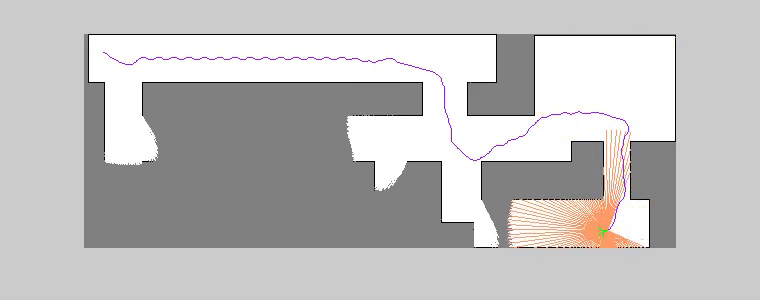
\includegraphics[width=4.5in]{whiskerbotstart.png}
\caption{MATLAB Simulation of a robot with a selection of three motion primitives, exploring an unknown environment.}
\label{fig:whiskerbotstart}
\end{figure}

\section{Hardware Test Platform}
We decided to use a ground robot instead of a quadrotor as our test platform because it has simpler dynamics and is safer to operate.
A ground robot (Figure \ref{fig:ground_robot}) has been equipped with a laser scanner to facilitate data collection.
It can be controlled by joystick as well as by an onboard controller.
We are fusing laser scans with IMU measurements to obtain state estimates to feed into the onboard controller.
Additionally, the ground robot's planner will be adapted from the quadrotor planner.

\begin{figure}[!htbp]
\centering
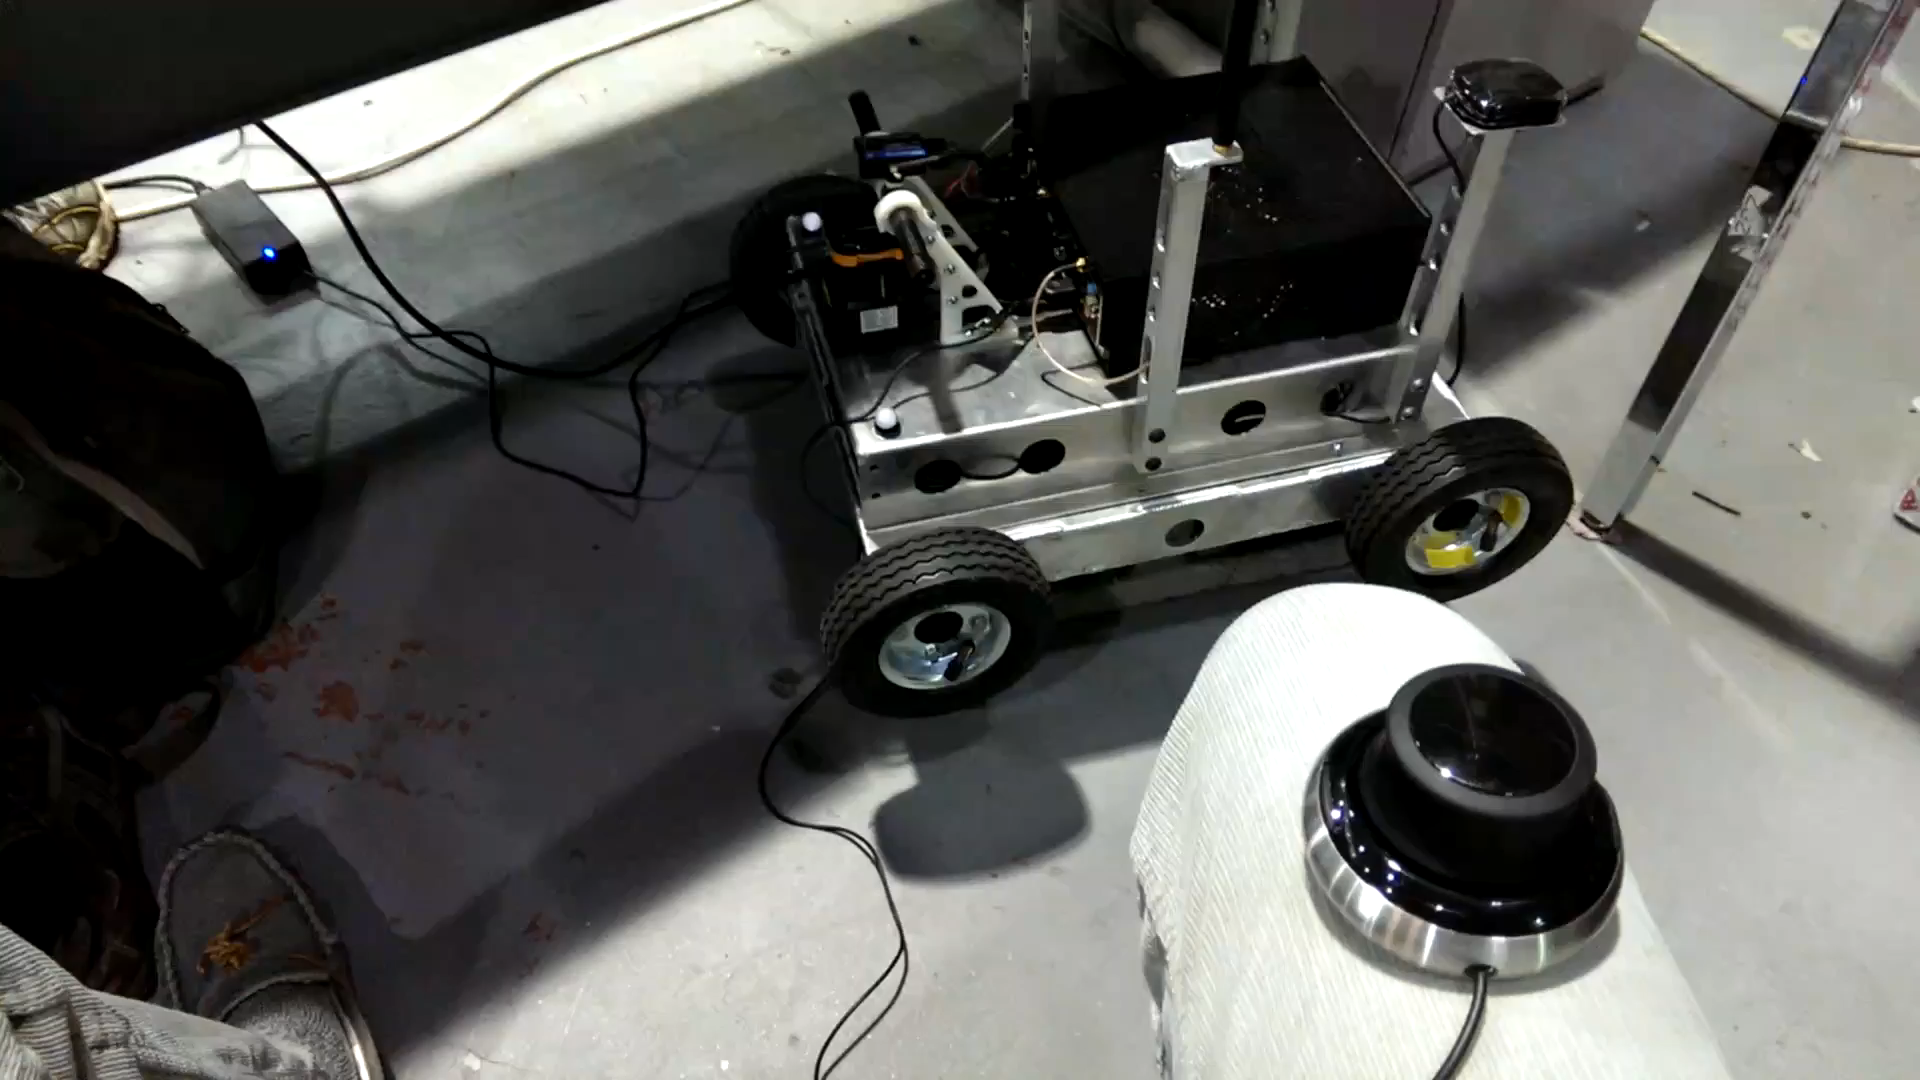
\includegraphics[width=4.5in]{ground_robot.png}
\caption{Ground robot equipped with laser scanner, IMU, and onboard computing.}
\label{fig:ground_robot}
\end{figure}


\end{document}








%\subsection{Subsection Heading Here}
%
%\begin{figure}[!t]
%\centering
%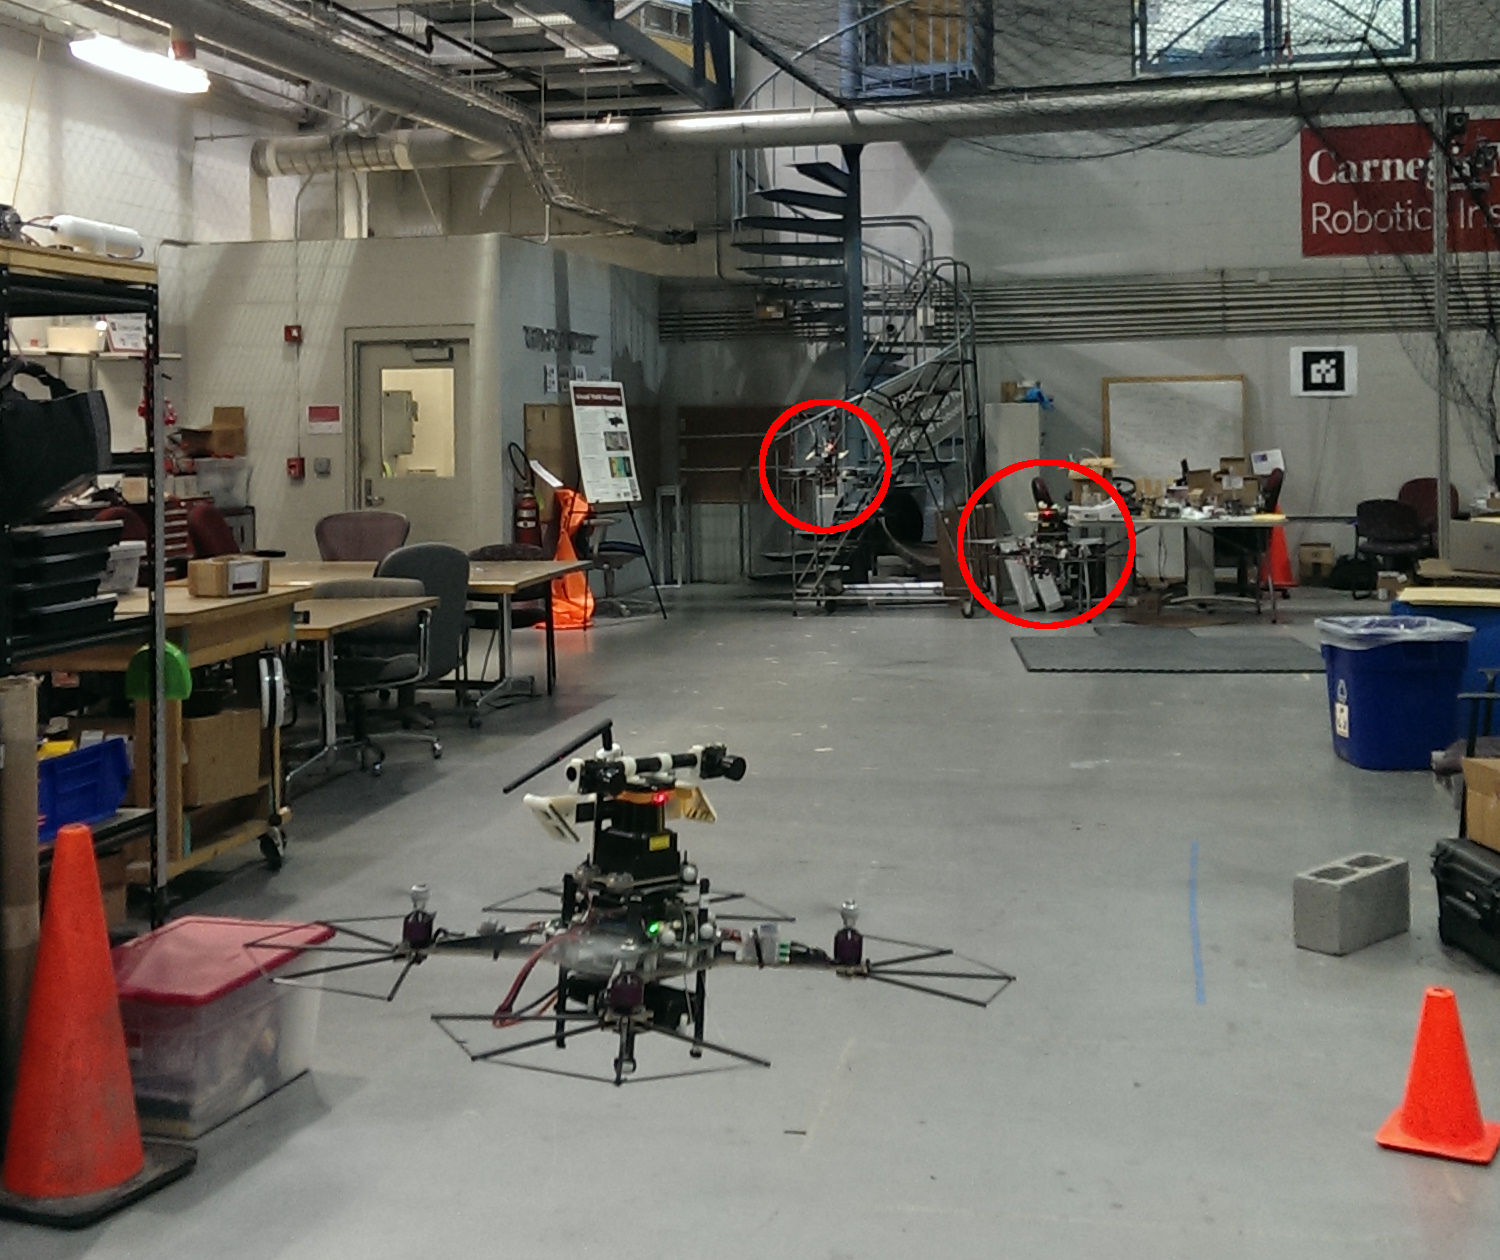
\includegraphics[width=2.5in]{3quads.png}
%\caption{Simulation Results}
%\label{fig_sim}
%\end{figure}
%\begin{table}[!t]
%\renewcommand{\arraystretch}{1.3}
%\caption{An Example of a Table}
%\label{table_example}
%\centering
%\begin{tabular}{|c||c|}
%\hline
%One & Two\\
%\hline
%Three & Four\\
%\hline
%\end{tabular}
%\end{table}

%\appendices
%\section{Proof of the First Zonklar Equation}

%\begin{thebibliography}{1}

%\bibitem{IEEEhowto:kopka}
%H.~Kopka and P.~W. Daly, \emph{A Guide to \LaTeX}, 3rd~ed.\hskip 1em plus
%  0.5em minus 0.4em\relax Harlow, England: Addison-Wesley, 1999.
%\end{thebibliography}
